\cotefile{84}
\scanpage{146}
% 146.01 Top line, left and centre
\[
T_1=\unsure{2,1_1|2\,1_1|2\cdot1_1},-b_1
=\deleted{\unsure{T_i}}\begin{pmatrix}2&0\\-b_1&0\end{pmatrix}
\qquad \unsure{R_1|\Pi_1|T_1|\bar T_1}=\begin{pmatrix}0&0\\b_1&2\end{pmatrix}
\]

% 146.02 Upper left, isolated mark and oval
\[
\deleted{\unsure{\xi_1|E_1}}\qquad
\tikz[baseline=(b.base)]\node[draw,ellipse,inner sep=2pt] (b) {$b=b_1b_2$};
\]

% 146.03 Upper left, three pairs and downward arrow
\diagram{\begin{tikzcd}[ampersand replacement=\&,column sep=small]
(E_1,\deleted{\unsure{\pi}}\deleted{\beta}\xi_1),(E_{\unsure{2|1}},\deleted{\beta}\xi_2)
 \arrow[r] \arrow[d,"\unsure{\mathrm{triv}|\mathrm{triv.}}"'] \& (E,\deleted{\beta}\xi)\ \text{\deleted{avec}}\\
 \deleted{b_1=E_1} \& \deleted{\unsure{E_1\longrightarrow}}
\end{tikzcd}}

% 146.04 Middle, separate indices over right-hand working
\[b_1\qquad b_2\]

% 146.05 Middle left, two composites
\diagram{\begin{tikzcd}[ampersand replacement=\&,column sep=small]
b_1\colon \deleted{E_1}M_1\arrow[r,"\tau_1^{\bullet}"] \& E_1\arrow[r,"\pi_1"] \& L_1\\
-b_1\colon M_1\arrow[r,"\varpi_1"] \& E_1\arrow[r,"\tau_{1\bullet}"] \& L_1
\end{tikzcd}}

% 146.06 Middle right, two pairs of changes and a membership
\[
\begin{aligned}
\unsure{\xi'_1|\tau'_1}&=\deleted{\unsure{\beta}}\xi_1+u_1 \ \big/ \ \xi'_{\unsure{1|2}}=\xi_2+u_2\\
b'_1&=b_1+\chi u_1\ \big/ \ b'_2=b_2+\chi u_2\\[-2pt]
&u_i\in\mathrm{Hom}(M_i,L_i)
\end{aligned}
\]

% 146.07 Below left composite, two lines
trivialisations $\xi$

\unsure{semi-trivialisations|pseudo-trivialisations} $\beta$

% 146.08 Lower left, two evaluations
\[
\begin{aligned}
\unsure{b_{\beta_2}|b\beta_2}\quad \beta_{\unsure{\bullet|*}}(\xi)&=b\in\mathrm{Hom}(M_1,L_1)\\
\beta^{\unsure{\bullet|*|\prime}}(\unsure{g|\xi|\eta})&=-b
\end{aligned}
\]

% 146.09 Lower centre, two mappings
\[
\begin{aligned}
x_1&\longrightarrow\pi_1(\tau_1^{\bullet}(x_1))\\
x_1&\unsure{\mathrel{\vdash}|\longmapsto}\pi_1(\tau_1^{\unsure{\prime|\bullet|}}(x_1)+u_1(x_1))
=\pi_1(\unsure{\tau_i|\tau_1}(x_1))
\end{aligned}
\]
% archive sheet number: 145
\scanpage{147}
% 147.01 Top centre
\mspage{475}

% 147.02 Upper half, paragraph 1
Si quelque chose ici sort du \unsure{.commun|commun}, ce n'est pas bien sûr la simple p\,r\,é\,s\,e\,n\,c\,e de ce double mécanisme, ni non plus (il me semble) la force de la composante ``répressive'' à proprement parler, la force donc de la répression des traits, attitudes, pulsions ``yin''. Il n'y a pas de commune mesure ici avec ce qui avait lieu chez ma mère, dont la vie (et celle de ses proches) a été dévastée par sa haine (restée occulte sa vie durant) de ce qui faisait d'elle une femme. A aucun moment, je crois, mes façons d'être n'ont été entièrement exempte d'une certaine douceur, voire de tendresse, qui obstinément arrondissaient les angles du personnage que je m'étais taillé depuis mon enfance, et qui \unsure{m'attiraie|m'attiraient} souvent sympathie et affection. Le côté exceptionnel se trouverait plutôt dans \unsure{l|la} d\,é\,m\,e\,s\,u\,r\,e de mes investissements, dans la démesure de l'énergie que j'investis dans mes tâches, sans m'en laisser distraire par un regard à droite ni à gauche! En dehors du travail proprement dit, mon esprit continuellement est projeté vers l'accomplissement, vers l'aboutissement de telle ou telle étape du travail. Cette attitude-là (``Zielgerichtetheit'' en allemand, ``aimdirectedness'' en anglais) est par excellence une attitude yang, une attitude de t\,e\,n\,s\,i\,o\unsure{:|}\,n, de f\,e\,r\,m\,e\,t\,u\,r\,e à tout ce qui n'apparaît pas directement lié à la tâche

% 147.03 Middle to lower half, paragraph 2
Cette démesure était de nature à susciter en autrui l'image d'une sorte de ``super-man'' ou ``super-mâle'', admirable certes hélas! (vu les valeurs qui ont cours), mais suscitant aussitôt (à un niveau qui reste inconscient le plus souvent) d'instinctives réactions de défense voire d'antagonisme devant un tel déployement de force, ressenti comme menaçant voire agressif, ou en tous cas dangereux (\({}^{108}2\)). Et surtout, cette image irresistiblement évoque l'image du ``s\,u\,p\,e\,r\,-\,p\,è\,r\,e'', et met en branle aussitôt la multiplicité ambigüe des réactions d'attraction et de répulsion nouées autour\unsure{:|} du sempiternel conflit au père... C'est là \unsure{:|}m\,a contribution dans ces relations d' a\,m\,b\,i\,g\,u\,i\,t\,é, qui ont été si communes dans ma vie, et auquelles je me suis retrouvé confronté tant de fois au cours de Récoltes et Semailles. Cette ambiguité est renforcée, non diminuée, par la persistance de traits yin en moi qui alimentent une sympathie, que la seule hypertrophie des traits yang en une sorte de gigantesque ``superman'' serait impuissante à susciter.

% 147.04 Bottom, paragraph 3
Et à nouveau je peux constater, dans ces sempiternelles ``relations d'ambiguité'', que je ne fais encore que récolter ce que j'ai moi-même semé, même si à chaque fois la récolte s'avère inattendue (et ma\handwritten{l}venue...)! Car la motivation (\unsure{o|ou} du moins u\,n\,e des motivations) qui pousse ``le patron'' en moi à se dépasser sans cesse dans l'accumulation des oeuvres, n'a-t-elle pas été justement de \unsure{forc|forcer} et relancer sans cesse l'estime de mes pairs (en premier lieu) et de mes impairs
% archive sheet number: 146
\scanpage{148}
% 148.01 Top left, first two lines
\[
\begin{aligned}
\sigma_1&=\mathrm{id}_1-\unsure{\gamma|r}\pi_1\\
\sigma_2&=\mathrm{id}_2-\gamma\pi_2
\end{aligned}
\]

% 148.02 Top right beside the vertical rule
\[
\begin{aligned}\beta_1&=\beta_2=1-\gamma\chi\\
\alpha&=-\chi(1-\gamma\chi)\end{aligned}
\qquad
\boxed{\gamma\chi=2}\quad
\boxed{\begin{aligned}\beta&=-1\\\alpha&=\chi\end{aligned}}
\]

% 148.03 Upper left, expansion with interlinear addition
\[
\begin{aligned}
\mathrm{id}_{12}+\sigma_1\otimes\sigma_2
 &=\inserted{\mathrm{id}_{12}+}\mathrm{id}_{12}-\gamma(\pi'_1+\pi'_2)+\gamma^2\pi_1^{\unsure{\prime}}\otimes\pi_2^{\unsure{\prime}}\\
 &=2\,\mathrm{id}_{12}-\gamma(\pi'_1+\pi'_2)+\gamma^2\pi'_1\otimes\pi'_2
\end{aligned}
\]

% 148.04 Upper middle, cancelled line
\[\deleted{\sigma_1=\alpha_1+\beta_1\pi_1}\]

% 148.05 Upper middle, below cancellation
\[\sigma_i=\lambda\,1_i+\mu\,\pi_i\]

% 148.06 Midpage, full-width expansion
\[
\mathrm{id}+\sigma_1\otimes\sigma_2=
\underbrace{\mathrm{id}_{12}+\lambda^2\mathrm{id}_{12}}_{(1+\lambda^2)\mathrm{id}_{12}}
+\lambda\mu(\pi'_1+\pi'_2)+\mu^2\pi'_1\otimes\pi'_2
\]

% 148.07 Middle left, three braced conditions
\[
\left\{\begin{aligned}\lambda^2+1&=\chi\\
\lambda\mu&=-1\\
\mu^2&=\gamma.\end{aligned}\right|
\]

% 148.08 Middle below rule, two short lines and two values
$u_i$ \unsure{endomorph. de|endomorphe de|échange de} \deleted{$\unsure{B}$}$E_i$ \unsure{i.e. élémts de}
\[
\begin{aligned}
\unsure{\mathscr H_i|H_i|\mathcal H_i}&=\text{\unsure{espace de|espace des}}\\
&\qquad 1,0
\end{aligned}
\]

% 148.09 Lower left, first row
\diagram{\begin{tikzcd}[ampersand replacement=\&,column sep=small]
0\arrow[r,dash]\&L\arrow[r]\&E\&[-1em]\unsure{\longleftarrow|\mathord{-}|\longrightarrow}\&[-1em]M\arrow[r,dash]\&0
\end{tikzcd}}

% 148.10 Lower left, second row
\diagram{\begin{tikzcd}[ampersand replacement=\&,column sep=small]
0\arrow[r]\&\mathrm{Hom}(M,L)\arrow[r,"\deleted{\unsure{k}}" description]\&\mathscr H/\mathrm{id}\arrow[r]\&\dfrac{\mathcal O\times\mathcal O}{\mathcal O}\arrow[r]\&0
\end{tikzcd}}

% 148.11 Lower right, short row
\diagram{\begin{tikzcd}[ampersand replacement=\&,column sep=small]
{}\arrow[r]\&\mathscr H\arrow[r]\&\underline{\mathcal O}\arrow[r,dash]\&{}
\end{tikzcd}}

% 148.12 Lower right, two equations
\[
\begin{aligned}
\sigma(\unsure{x|u})&=(\lambda(u)+\mu(u))(\mathrm{id})-u\\
u+\sigma(u)&=(\lambda(u)+\mu(u))\,\mathrm{id}
\end{aligned}
\]

% 148.13 Foot, left, upward map
\diagram{\begin{tikzcd}[ampersand replacement=\&]
\unsure{i}\\[-2pt]
\mathrm{Hom}(M\otimes M',L\otimes L')\\
\mathrm{Hom}(M,L)\otimes\mathrm{Hom}(M',L')\arrow[u]
\end{tikzcd}}
% archive sheet number: 147
\scanpage{149}
% 149.01 Top centre
\mspage{47\handwritten{5 bis}}

% 149.02 Upper quarter, continuation
(par surcroît); d'entendre certains des meilleurs se lamenter qu'ils ne peuvent me suivre, au rythme où je cours de l'avant ?! Oui, il y a bien eu en moi ce secret désir de susciter en autrui (comme en moi-même) cette image ``plus grande que nature'', démesurée comme celui-là même qu'elle reflète - et qui obstinément me revient à travers l'autre: en paroles claires et hautes, par l'éloge escompté (et encaissé comme un dû) - et a\,u\,s\,s\,i , par les voies obscures et \unsure{profond|profondes} de l'inimitié sourde et du conflit...(*)

% 149.03 Foot, below short rule
\noindent\rule{5em}{0.3pt}\par
(*) (6 octobre) Pour tout dire, ``ce secret désir'' sur lequel je viens de mett\deleted{\unsure{e}}\handwritten{re} à nouveau le doigt, n'est pas consumé aujourd'hui encore, même s'il a été décelé enfin (depuis quelques années à peine...), et s'il est moins dévorant aujourd'hui que jadis.
% archive sheet number: 148
\scanpage{150}
% 150.01 Top line, crossed obliquely
\deleted{Mais \unsure{je|on} veux \unsure{compatibilité} avec les \unsure{$\pi$|$R$}-\unsure{trivialisations}.}

% 150.02 Upper left, crossed downward map
\diagram{\begin{tikzcd}[ampersand replacement=\&]
\deleted{E_1\vee E_2}\arrow[d,"\deleted{\pi_{E_1\vee E_2}}"]\\{}
\end{tikzcd}}

% 150.03 Upper centre, oval
\[
\tikz[baseline=(s.base)]\node[draw,ellipse,inner sep=2pt] (s) {$x_1\otimes x_2+\overline{x}_1\otimes\overline{x}_2$};
\]

% 150.04 Upper right, under oval
\[(x_1-\pi_1(x_1))(x_2-\pi_2(x_2))\]

% 150.05 Middle, double-bar calculation and work below brace
\[
\overline{\overline{x_1}}=\deleted{\unsure{x_1\otimes|x_1\,0|x_1,0}}(x_1-\pi_1(x_1))
-\underbrace{\pi_1(x_1-\pi_1(x_1))}_{-\pi_1(x_1)+\underset{\substack{\shortparallel\\2}}{\chi}\pi_1(x_1)}=x_1
\]

% 150.06 Middle, line starting with x
$x_1\unsure{\mathbin{-}|\mapsto}\overline{x}_1$ \unsure{induit} $-\mathrm{id}$ sur $L_1$, $+\mathrm{\unsure{id|Id}}$ sur $M_1=E_{\unsure{11|1}}/L_1$

% 150.07 Lower right, two equations and isolated values
\[
\begin{aligned}\pi^{\unsure{2|\prime}}-\chi\pi&=0\\
\pi(\pi-\chi)&=0\\ &\qquad 0\quad\chi\end{aligned}
\]

% 150.08 Lower left, two lines
\[
\begin{aligned}
&x_1-\varpi_1(x_1)\qquad \varpi_1(x_1)=2x_1-\pi_1(x_1)\\
&=x_1-(2x_1-\pi_1(x_1))=\pi_1(x_1)-x_1=-\overline{x}_1
\end{aligned}
\]

% 150.09 Foot, bracket under first two terms
\[
\tikz[baseline=(a.base)]{\node[inner sep=1pt] (a) {$(\chi-1)\mathrm{id}+(1_1-\pi_1)\otimes(1_{1}-\pi_2)$};\draw (a.south west) -- ++(0,-2pt) -| (a.south east);}
+(\unsure{\gamma|r}-1)\pi_1\otimes\pi_2
\]
% archive sheet number: 149
\scanpage{151}
% 151.01 Top centre
\mspage{478}

% 151.02 Upper paragraph
D'ailleurs, comme revers de l'aisance dont je parle, j'ai tendance souvent à sous-estimer la difficulté que peut présenter pour tel élève l'acquisition de tel bagage, ou le développement de tel outil - ce qui a tendance à le placer en porte-à-faux vis à vis de mes expectatives. (Voir à ce sujet la note ``Echec d'un enseignement (1)'', n\textsuperscript{o} 23 iv.) Une telle situation doit assez souvent être un des ingrédients importants d'une relation fausse au père...

% 151.03 Middle, note 109
(\textsuperscript{109}) (9 octobre) Je me suis senti tout content, en terminant la note précédente (*), il y a quatre jours. Je me suis trouvé inopinément renouer avec une intuition qui m'était venue un certain dimanche 17 octobre 1976 (il va y avoir huit ans à quelques jours près) - l'intuition de l'effet dévastateur, dans ma \unsure{vie|vi} comme dans celle de ma mère, d'une ``certaine force'' en moi. C'était la première fois de ma vie que je consacrais une réflexion, si sommaire soit-elle, à ce qu'avait été ma vie et surtout, mon enfance. C'était aussi le surlendemain du jour où j'avais découvert le pouvoir de méditation (**), et c'était la première fois depuis ce moment que je faisais usage de ce pouvoir, si longtemps ignoré. C'est sans propos délibéré, par l'effet d'une impulsion profonde, comme mû par un instinct très sûr, que la réflexion ce jour-là a fini par se diriger vers mon enfance. Avec le recul seulement, je mesure à quel point c'était bien à la source de ma vraie force, comme aussi du conflit et de la division en moi, que m'avait porté alors un besoin profond de connaître. Pendant près de trois \unsure{an|ans} je n'allais plus y revenir, distrait que j'étais pendant ces années par les \unsure{seul|seules|seuls} questions ``d'ordre du jour'', sans me rendre compte que je restais à la \unsure{périphéri|périphérie} du conflit dans ma vie, tout en me tenant obstinément éloigné du coeur même: de cette enfance noyée de brumes, qui paraissait si infiniment lointaine...

% 151.04 Lower paragraph, ends at page break
Je viens de parcourir à nouveau, ``en diagonale'', les dix huit feuilles, d'une densité exceptionelle, de cette méditation cruciale dans ma vie. C'est dans la nuit qui a suivi cette méditation, ou plutôt au petit matin après cette nuit de méditation, que j'ai eu un rêve d'une force bouleversante - le premier rêve aussi dans ma vie dont j'aie sondé le message, passionnément. Je ne me rendais pas plus compte alors où j'allais et de ce qui était en train de se passer, que l'avant-veille quand j'étais en train de ``découvrir la méditation''. Du-

% 151.05 Foot, first note below rule
\noindent\rule{5em}{0.3pt}\par
(*) Voir la note ``Yang enterre yin - ou le Super père'', n\textsuperscript{o} 108.

% 151.06 Foot, second note
(**) Voir la section ``Désir et méditation'', n\textsuperscript{o} 39.
% archive sheet number: 150
\scanpage{152}
% 152.01 Top left and centre, parameters
\[
\underbrace{\beta_1=\beta_2}_{\beta}=1-\underline{\underline{\underline{\unsure{\gamma|r}}}}\chi
\qquad \alpha=-\beta\deleted{\unsure{\gamma}}\chi=-\chi(1-\underline{\underline{\underline{\gamma}}}\chi)
\]

% 152.02 Upper line, operator and integer condition
\[
-\chi(1-\underline{\gamma}\chi)\mathrm{id}+(1-\gamma\chi)(\pi'_1+\pi'_2)+\gamma\pi'_1\otimes\pi'_2
\qquad\gamma\in\mathbb Z
\]

% 152.03 Next line, evaluation and check
\[
-\chi\underline{(1-\gamma\chi)}+2(1-\gamma\chi)\chi+\gamma\chi^2=\chi
\qquad\deleted{2\chi=\chi}\quad\chi=\chi\quad\text{O.K.!}
\]

% 152.04 Left below evaluation, cancelled box
\[\deleted{\boxed{2=\chi}}\]

% 152.05 Middle right, two-line operator
\[
\begin{aligned}
&-\chi\cdot(1-\gamma\chi)\,\mathrm{id}_{M_1\otimes M_2}
+(\deleted{\unsure{\pi}}1-\gamma\chi)[(\tau_1\otimes\mathrm{id}_2)+\mathrm{id}_1\otimes\tau_2]\\
&\hspace{12em}+\deleted{\unsure{x_1\otimes x_2}}\gamma\,\tau_1\otimes\tau_2
\end{aligned}
\]

% 152.06 Lower middle, braced conditions and boxed product
\[
\left\{\begin{aligned}-\chi(1-\gamma\chi)&=\chi\\1-\gamma\chi&=-1\end{aligned}\right.
\qquad
\begin{aligned}1-\gamma\chi&=-1\\\boxed{\gamma\chi=2}\end{aligned}
\]

% 152.07 Right of box, two lines
\unsure{OK si|ok si} $\chi=\pm2$

\unsure{si} $\chi$ \deleted{$\unsure{\chi}$}

% 152.08 Lower left to right, choice of parameters
$\chi=2\qquad\gamma=1,\ \beta=-1,\ \alpha=2$ \unsure{donc on prend}

% 152.09 Lower right, chosen operator
\[
\curvearrowleft\ \curvearrowright\quad\deleted{2\,\mathrm{id}}\quad
2\,\mathrm{id}_{E_1\otimes E_2}-
(\pi_{E_1}^{\unsure{\prime|}}\otimes\mathrm{id}_{E_2}+\mathrm{id}_{E_1}\otimes\pi_{E_2})
+\pi_{E_1}\otimes\pi_{E_2}
\]

% 152.10 Lower right, image of a tensor and struck equivalent
\[
\begin{aligned}
x_1\otimes x_2&\longmapsto 2x_1\otimes x_2-\pi_1(x_1)\otimes x_2-x_1\otimes\pi_2(\unsure{x_1|x_2})\\
&\hspace{12em}+\pi_1(x_1)\otimes\pi_2(\unsure{x_1|x_2})\\
&\deleted{\equiv x_1\otimes x_2+(\overline{x}_1\otimes\overline{x}_2)}
\end{aligned}
\]

% 152.11 Foot left, two identities
\[
\begin{aligned}
\overline{x}_1&=T_1\psi_1(x_1)-x_1=x_1-\pi_1(x_1)\\
\pi_1(x_1)&=2x_1-T_1\psi_1(x_1)
\end{aligned}
\]
% archive sheet number: 151
\scanpage{153}
% 153.01 Top centre
\mspage{476}

% 153.02 Top paragraph, note 108 with following 1
(\textsuperscript{108}1) (6 octobre) Je veux dire que les forces de nature répressive qui ont joué dans ma vie, semblent prendre surtout, sinon exclusivement, l'une de ces deux formes spécifiques: enterrement du passé, et mise en avant de mes traits ``virils au détriment de mes traits ``féminins''. Je n'entends nullement dire que ces deux ``forces'', de nature répressive l'une et l'autre (c'est à dire, visant à un ``refoulement'', à un escamotage d'une certaine réalité), soient les seules qui aient ``dominé ma vie''! Ce serait oublier tout l'aspect non égotique de mon être, la pulsion de connaissance s'exprimant aussi bien au niveau de corps que de \unsure{l'espri|l'esprit} (Voir à ce sujet notamment ``Mes passions'', section n\textsuperscript{o} 35.)

% 153.03 Middle paragraph
Même parmi les forces stucturant le moi, émanation du ``patron'' donc, il en est au moins une, de nature non répressive par elle-même, bien antérieure aux forces de répression et dont le rôle dans ma vie a été plus essentiel encore: c'est l'identification à mon père, qui a été comme ``le coeur paisible et \unsure{puissan|puissant} du sentiment de ma propre force. Cette identification n'allait nullement dans le sens de l'exaltation de certaines valeurs ou qualités (viriles disons) au détriment d'autres (``féminines''). Indépendamment des valeurs professées par mon père, sa personne (jusqu'en 1933, où un basculement a eu lieu en lui (*)), a été empreinte d'un fort équilibre yin-yang, où l'intuition et la spontaneité n'avaient pas une moindre part que l'intellect et la volonté.

% 153.04 Lower paragraph
Enfin, comme autre ``force'' importante de nature égotique, intimement liée, elle, aux mécanismes répressifs (ou pour mieux dire, de nature ``répressive'' elle-même), il convient encore de compter la sempiternelle v\,a\,n\,i\,t\,é , dont le rôle a été aussi lourd dans ma vie que dans celle de quiconque. Mais cette ``force''-là est de nature si universelle, tout comme le rôle dominant qu'elle joue dans la vie de chacun (sous une forme plus ou moins grossière ou subtile), qu'il n'y a guère lieu de l'inclure expressément, dans un relevé des formes spécifiques que prennent chez une personnne les forces et mécanismes qui structurent le moi, et donnent à celui-ci sa physionomie particulière et son assise.

% 153.05 Footnote below rule
\noindent\rule{5em}{0.3pt}\par
(*) Chose remarquable\handwritten{,} ce ``basculement'' chez mon père (agé alors de 43 ans) s'est fait vers un état s\,u\,p\,e\,r\,-\,y\,i\,n , vers une sorte de passivité de pacha, en étroite connivence avec ma mère, jouant un rôle super-yang. Celle-ci l'a pris en charge \hspace{1em} lieu et place de ses enfants.(Ils sont largués aux ``profits et pertes'', jusqu'en 1939 tout au moins, l'année où sous la pression des évènements et à son corps défendant, elle finit par me reprendre auprès d'elle...) Cette relation de dépendance de mon père et de renversement des rôles yin-yang entre mes parents, a duré jusqu'à la disparition de mon père en 1942.
% archive sheet number: 152
\scanpage{154}
% 154.01 Top, cancelled tensor and four terms with overlapping braces
\[
\deleted{E_1\otimes E_2}\quad
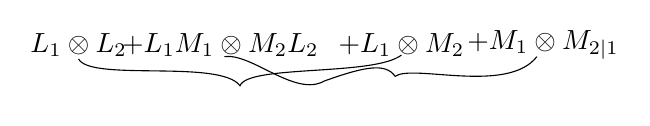
\begin{tikzpicture}[baseline=(a.base)]
\node[inner sep=1pt] (a) at (0,0) {$L_1\otimes L_2$};
\node[inner sep=1pt] (b) at (1.8,0) {$+\deleted{L_1}M_1\otimes\deleted{\unsure{M_2}}L_2$};
\node[inner sep=1pt] (c) at (4.1,0) {$+L_1\otimes M_2$};
\node[inner sep=1pt] (d) at (5.9,0) {$+M_1\otimes M_{\unsure{2|1}}$};
\draw (0,-.18) .. controls (.15,-.47) and (1.8,-.18) .. (2.05,-.52) .. controls (2.15,-.25) and (3.75,-.4) .. (4.1,-.13);
\draw (1.85,-.15) .. controls (2.2,-.1) and (2.75,-.67) .. (3.12,-.46) .. controls (3.65,-.27) and (3.9,-.23) .. (4.02,-.4) .. controls (4.24,-.24) and (5.45,-.63) .. (5.82,-.15);
\end{tikzpicture}
\]

% 154.02 Upper left, diagram in three levels
\diagram{\begin{tikzcd}[ampersand replacement=\&,column sep=small,row sep=small]
E_1\otimes_{0}E_2\arrow[rr,"F_{11}^{!}"]\arrow[dr,"\pi"]\arrow[dd]\arrow[ddrrr,bend right=30,dash]
\&{}\&E_1\otimes E_2\arrow[rr]\&{}\&E_1\otimes^{0}E_2\\
{}\&L_1\otimes L_{\unsure{2|12}}\arrow[ur,"\alpha_1\otimes\alpha_2"']\&{}\&\text{\deleted{\unsure{confusi|conveni|connu}\,\unsure{ment|avec|}}}\&{}\\
E_1\otimes\unsure{E_2|\Omega}\arrow[rrr,dash,"\psi_1\otimes\psi_2"']\&{}\&{}\&M_1\otimes M_2\arrow[uur]\&{}
\end{tikzcd}}

% 154.03 Upper right, two factors
\[(E_1\otimes M_2)\times(M_1\otimes E_2)\]

% 154.04 Above table, three objects
\diagram{\begin{tikzcd}[ampersand replacement=\&]
L_1\otimes L_2\arrow[r,dash]\&\otimes\arrow[r,dash]\&\otimes
\end{tikzcd}}

% 154.05 Immediately above table
\[\unsure{\mathbb Z|\xi}\]

% 154.06 Centre, four by four table
\diagram{$\begin{array}{c|cccc}
 &L_1\deleted{\unsure{\otimes}}\otimes L_2 & L_1\otimes M_2 & M_1\otimes L_2 & M_1\otimes M_2\\ \hline
L_1\otimes L_2 &\chi&\mathrm{id}_{L_1}\otimes\tau_2&\tau_1\otimes\mathrm{id}_{L_2}&?\ (T_1\otimes T_2\,?)\\
L_1\otimes M_2 &0&0&0&\underline{?}\ \cdot\tau_1\otimes\mathrm{id}_{M_2}\\
M_1\otimes L_2 &0&0&0&\underline{?}\ \deleted{\unsure{\tau_2}}\mathrm{id}_{M_1}\otimes\tau_2\\
M_1\otimes M_{1} &0&0&0&\chi
\end{array}$}

% 154.07 Below table, three lines and right-hand addition
On \unsure{trouve} que les 2 \deleted{\unsure{compositions}}\inserted{\unsure{homomorphismes de}} \unsure{carré|coïnc.|connues}\inserted{ sur $E_{\unsure{11|12}}$} sont compatibles, et laissent une \unsure{indétermination|indéterminée}, qui est un hom de $M_1\otimes M_2$ en $L_1\otimes L_2$.

% 154.08 Lower centre, two columns of working
\[
\begin{aligned}
-\qquad E_1\otimes E_2 &\qquad E_1\otimes E_2\\
\pi'_1=\alpha_1\pi_1\ \big/\ \unsure{\omega'_1|\varpi'_1}=\varpi_1\psi_1&\qquad \pi'_1+\varpi\\
\pi'_2=\alpha_2\pi_2\qquad\varpi'_2=\omega_2\psi_2&
\end{aligned}
\]

% 154.09 Foot, three lines
C'est normal, car pour l'instant on n'a \unsure{rien|écrit} \uline{que} le fait qu'on veut une \unsure{iso|paire|loi} d'extensions - \deleted{\unsure{et}} celles-ci sont \unsure{triviales|toutes}, on a l'embarras du choix !
% archive sheet number: 153
\scanpage{155}
% 155.01 Top centre
\mspage{479}

% 155.02 Top, continued word
rant quatre heures je me suis enfoncé dans le sens de ce vécu-là, de ce rêve-parabole, à travers des couches successives de signification de plus en plus brûlantes, avant d'arriver au coeur du message, à son sens simple et evident.

% 155.03 Second paragraph, above gap
Ce n'a pas été alors le déclic subit d'une compréhension de ``l'intelligence''\handwritten{,} ni même comme une lumière subite dans une obscurité ou dans une pénombre. C'était plutôt comme une vague profonde née en moi et qui soudain déferlait à travers moi et dans ses vastes eaux m'apportait ce sens qui s'était dérobé jusque là: que je retrouvais en ce moment un être très cher et très précieux, que j'avais perdu depuis mon enfance...

% 155.04 Middle paragraph, below gap
Ce moment a été vécu comme une n\,a\,i\,s\,s\,a\,n\,c\,e , comme un renouvellement profond. Ce sentiment est resté très fort toute cette journée\handwritten{,} et encore dans les jours suivants. Avec le recul de huit ans, ce moment m'apparaît aujourd'hui encore comme un moment créateur entre tous dans ma vie, et celui d'un tournant essentiel dans mon aventure spirituelle. Il a été préparé certes par bien d'autres ``moments'', dans les jours et dans les mois qui avaient précédé. Le premier précurseur peut-être a été cet ``arrachement salutaire'', plus de dix ans auparavant, d'une institution où je comptais bien finir mes jours (*). Ces moments antérieurs m'apparaissent un peu comme les ingrédients, ou plutôt comme les m\unsure{\textperiodcentered|}\,o\,y\,e\,n\,s à ma disposition, avec lesquels je pouvais franchir cet autre ``seuil'' qui était devant moi sans que je l'aperçoive, qui se situait à un niveau plus profond, plus caché que d'autres que j'avais franchis. Tout était réuni, depuis quelques jours ou heures, pour que je le franchisse - et je pouvais le franchir, comme je pouvais ne pas le franchir, jour après jour ma vie durant..

% 155.05 Lower paragraph
Et aussi, ce seuil étant bel et bien franchi, la voie s'est trouvée ouverte vers d'autres franchissements encore, vers d'autres ``éveils'' ou ``réveils'', dont chacun par nature est aussi un renouvellement, et tant soit peu, une \unsure{:|}``nouvelle naissance'', une re-naissance. Il m'est arrivé d'en éluder certains des mois voire des années durant, pour finir par franchir le pas, m'allégeant au passage de quelque illusion tenace, qui une vie durant s'était interposée entre moi et la pleine saveur de ma vie et du monde qui m'entoure. Et sûrement aussi, il en est que je continue à éluder, au moment encore où j'écris ces lignes...

% 155.06 Footnote below rule
\noindent\rule{5em}{0.3pt}\par
(*) Voir la note n\textsuperscript{o} 42, de même nom.
% archive sheet number: 154
\scanpage{156}
% 156.01 Top, cancelled opening and isolated sign
\[
\begin{aligned}
&\deleted{-\chi(1-\delta\chi)}\\
&\unsure{\xi|\in}
\end{aligned}
\]

% 156.02 Top, large box
\[
\boxed{\begin{aligned}
&-\chi(1-\delta\chi)x_1\otimes x_2+(1-\delta\chi)[x_1\otimes\pi_2(x_2)+\pi_1(x_1)\otimes x_2)\\
&\hspace{12em}+\delta\,\pi_1(x_1)\otimes\pi_2(x_{\unsure{2|1}})
\end{aligned}}
\]

% 156.03 Below box, chosen coefficient
Si $\deleted{\unsure{\beta}}\chi=2$, on peut prendre $\delta=1$

% 156.04 Upper middle, two coefficient lines
\[
\begin{aligned}
\text{\unsure{donc|alors}}\qquad\alpha&=-2(1-2)=2\\
\beta=\unsure{\gamma|r}&=1-2=-1
\end{aligned}
\]

% 156.05 Middle, line to right edge
\[
\text{\unsure{donc|d'où}}\qquad
2x_1\otimes x_2-[(x_1\otimes\pi_2(x_2)+\pi_1(x_1)\otimes x_2)]
+\pi_1(x_{\unsure{1}})\otimes\pi_2(x_{\unsure{2}})
\]

% 156.06 Middle, cancelled identity
\[\deleted{\pi_i(x_i)=2x_i-T_i\psi(x_i)}\]

% 156.07 Middle to lower, identity and bar
\[
\begin{aligned}
\pi_i(x_i)&=2\unsure{x_i|\alpha_i}-T_i\psi_i(x_i)=2x_i-(x_i\unsure{+|-}\bar x_i)\\
&&{}\deleted{\unsure{x_i}}-\bar x_i\\
\bar x_i&=T_i\psi_i(x_i)-x_i\quad\deleted{\unsure{=x}}\\
x_i+\bar x_i&=T_i\psi_i(x_i)
\end{aligned}
\]

% 156.08 Lower middle, bracketed expansion
\[
\begin{aligned}
&2x_1\otimes x_2-\big[(\underline{x_1\otimes(x_2}-\bar x_2)+(\underline{x_1-\bar x_1)\otimes x_2})\big]
+(\underline{x_1-\bar x_1)\otimes(x_2}-\bar x_2)\\
&\qquad=x_1\otimes x_2+\bar x_1\otimes\bar x_2\qquad\text{O.K.}
\end{aligned}
\]

% 156.09 Foot, unfinished brace
\[\bar x_i=x_i-\pi_i(x_i)=\big\{\]

% 156.10 Foot, partial product and cancellation
\[x_1\otimes x_2+\deleted{(x_i-\unsure{\pi_i|R_i}(x)}\]

% 156.11 Bottom, question, reduction and boxed relation
\[
\begin{aligned}
-\chi(1-\delta\chi)&\overset{?}{=}\chi\\
-1+\delta\chi&=1\qquad\boxed{\delta\chi=2}
\end{aligned}
\]
% archive sheet number: 155
\scanpage{157}
% 157.01 Top centre
\mspage{486}

% 157.02 Upper continuation
très fort auprès des femmes dont j'ai été amant par la suite, en réveillant en l'amante des pulsions masculines, qui durant toute sa vie avaient été soigneusemant refoulées, et n'avaient trouvé à s'exprimer jusque là qu'``à la sauvette'' comme des sortes de bavures, indignes de figurer dans le vécu amoureux conscient

% 157.03 Upper and middle paragraph
Le vécu amoureux inconscient est riche de pulsions archétypes, dont une \unsure{de|des} plus puissantes est celle du retour à la Mère, du retour dans le giron originel. Un tel archétype est présent dans les couches profondes de l'expérience amoureuse, chez l'homme et aussi chez la femme. En la femme, les résistances à la satisfaction d'une telle pulsion dans le vécu amoureux du couple sont plus fortes encore que chez l'homme, où elle se heurte à un tabou-clef, et non à deux comme chez elle. Chez l'un comme chez l'autre, la satisfaction de ces pulsions \unsure{\textperiodcentered|}dans le vécu commun reste souvent plus ou moins symbolique et surtout, dérobé à la conscience. Quand un tel archétype et ce vécu remontent des couches profondes jusqu'à la lumière du jour, dans le champ du regard conscient, ce vécu aussitôt se transforme, il acquiert une dimension nouvelle. En même temps se libèrent des énergies considérables, précédemment comprimées par les mécanismes répressifs, ou liées par les tâches de répression. L'effet est celui d'une l\,i\,b\,é\,r\,a\,t\,i\,o\,n immédiate de la pulsion érotique, se manifestant par une intensité renouvelée et par une plénitude nouvelle dans l'expérience amoureuse.

% 157.04 Lower paragraph, after gap
Par ce qui précède, il apparaîtra déjà, sûrement, que cette acceptation nouvelle de ma propre personne est allée de pair avec une acceptation d'autrui. L'un et l'autre sont indissolublement liés. Il est entendu qu'il s'agit ici d' ``acceptation'' dans le plein sens du terme, qui ne signifie nullement une t\,o\,l\,é\,r\,a\,n\,c\,e (souvent aigre-douce) vis-à-vis de tels et tels ``travers'' ou ``défauts'', ressentis comme un mal hélas inévitable, pour lequel on est bien obligé de ``faire avec''. Dans une telle attitude, je sens surtout une résignation, pour ne pas dire une abdication, et sûrement pas une source de joie, ni un élan de prise de connaissance d'une chose digne d'être connue: la profondeur préssentie\handwritten{,} inconnue, derrière la plate surface de tels ``défauts'' ou ``travers'' qu'on veut bien tolérer...

% 157.05 Bottom, incomplete paragraph
Qu'il s'agisse ici d'une acceptation joyeuse, créatrice, ne signifie nullement pour autant que cette acceptation soit totale\handwritten{-}hier déjà j'ai constaté qu'il n'en était rien. Un lecteur attentif l'aura déjà constaté par lui-même plus d'une fois au cours de Récoltes et Semailles, comme il m'est arrivé de m'en
% archive sheet number: 156
\scanpage{158}
% 158.01 Top, two cancelled starts
\[\deleted{\alpha u_1\otimes x_2+}\qquad\deleted{\alpha\unsure{u_1|\beta_1}+\chi\unsure{\gamma|r}}\]

% 158.02 Upper first expression and value underneath
\[
\begin{aligned}
&(\alpha+\chi\gamma)u_1\otimes x_2+(\beta\deleted{\unsure{x_1}}+\delta\chi)u_1\otimes\pi_2(x_{\unsure{2|1}})\\
&\hspace{11em}\shortparallel\\[-2pt]
&\hspace{10em}u_1\otimes\pi_2(x_2)
\end{aligned}
\]

% 158.03 Upper equation and quantified line
\[
\begin{aligned}
(\alpha+\chi\gamma)u_1\otimes x_2+(\beta+\delta\chi-1)u_1\otimes\pi_2(x_{\unsure{1|2}})&=0\\
\forall u_1\in L_{\unsure{1|2}},\ x_2\in E_2&
\end{aligned}
\]

% 158.04 Upper middle, specialization
Si $x_2=u_2$ on \unsure{trouve}

% 158.05 Below specialization, two cancellations
\[\deleted{\unsure{u_i|u_1}}\qquad(\alpha+\chi\gamma\deleted{+})+\chi(\beta+\delta\chi-1)=0\]

% 158.06 Middle, factored expression
\[u_1\otimes\underline{[(\alpha+\chi\gamma)x_2+(\beta+\delta\chi-1)\deleted{\unsure{\beta_2}}\pi_2(x_2)]}=0\]

% 158.07 Middle, line after bracket
Donc \unsure{dans|sur} $L'_2$ on a

% 158.08 Middle to lower, scalar equations
\[
\begin{aligned}
(\alpha+\chi\gamma)\,\mathrm{id}&=0\\
\text{donc}\qquad \alpha+\chi\gamma&=0\\
\alpha&=-\chi\gamma\\
\text{donc aussi}\qquad \alpha&=-\chi\beta\qquad\text{donc }\underline{\beta=\gamma}
\end{aligned}
\]

% 158.09 Lower middle, crossed expression
\[\deleted{\beta+\delta}\]

% 158.10 Lower, tensor expansion
\[
\begin{aligned}
&-\chi\beta x_1\otimes x_2+\beta(x_1\otimes\pi_2(x_2)+\pi_1(x_1)\otimes x_2)+\delta\pi_1(x_1)\\
&\hspace{22em}\otimes\pi_2(x_2)
\end{aligned}
\]

% 158.11 Near foot, preceding last condition
il reste \unsure{donc}

% 158.12 Bottom, cancellation, condition and box
\[
\begin{aligned}
&\deleted{\unsure{\pi_2(x_2)-1}\ \unsure{1\otimes1|\oplus(\beta}}\quad(\beta+\delta\chi-1)\pi_2(x_2)=0\\
&\boxed{\beta+\delta\chi=1}
\end{aligned}
\]

% 158.13 Bottom right, solution and cancelled continuation
\[
\begin{aligned}\beta&=1-\delta\chi.\\
\alpha&=-\chi\beta=\\ &\deleted{=\chi+\chi^2}\end{aligned}
\]

% 158.14 Bottom left, two lines against the edge
\[
\begin{aligned}\beta&=\deleted{\unsure{\beta}}\gamma=1-\delta\chi\\
\alpha&=-\chi(1-\delta\chi)\end{aligned}
\]
% archive sheet number: 157
\scanpage{159}
% 159.01 Top centre
\mspage{487}

% 159.02 Upper paragraph, continuation
rendre compte en passant, quand je me voyais confronté à nouveau à ce sempiternel mécanisme en moi de r\,e\,j\,e\,t de tout ce qui se présente sous une apparence déplaisante, chez autrui ou chez moi-même. (Mais quand il d'agit de soi-même, ce mécanisme le plus souvent a comme effet de ne pas même prendre connaissance de la chose déplaisante en question...)

% 159.03 Main paragraph
L'acceptation dont je parle prend racine dans un i\,n\,t\,é\,r\,ê\,t pour cette chose qu'on ``accepte'', chez soi-même ou chez autrui. Alors que l'acceptation est par elle-même une disposition intérieure de caractère typiquement ``yin''\unsure{:|,} cette connot\handwritten{a}tion d'``intérêt'' qu'elle prend chez moi est de nature ``yang'' - \unsure{c'es|c'est} le ``yang dans le yin'', dans la délicate dialectique chinoise de l'entrelacement à l'infini du yin et du yang... J'allais me hasarder à dire, un peu dans la foulée\handwritten{,} qu'il y avait une identité pure et simple entre l'acceptation (la vraie!) et cet intérêt, cette curiosité. Pourtant, en posant un peu sur la chose, je me rends compte qu'il y a bien aussi une autre façon d'accepter, de nature, elle, plus totalement yin que celle qui m'est surtout coutumière. C'est comme un a\,c\,c\,u\,e\,i\,l de la chose acceptée, et non un élan vers elle pour la sonder. (Cette nuance d'accueil m'apparaît du coup comme le ``y\,i\,n d\,ans le yin'', nous y voilà!) L'élan de l'intérêt, et l'attitude d'accueil, peuvent l'une comme l'autre former la note de fond de l'acceptation d'autrui ou de soi. La chose commune aux deux est la s\,y\,m\,p\,a\,t\,h\,i\,e . C'est là aussi une des formes de l' a\,m\,o\,u\,r . S'il y a quelque identité profonde à cerner ici, ce serait donc par la constatation que l\,'\,a\,c\,c\,e\,p\,t\,a\,t\,i\,o\,n e\,s\,t u\,n\,e f\,o\,r\,m\,e d\,e l\,'\,a\,m\,o\,u\,r . Amour de soi, amour de l'autre, l'un et l'autre indissolublement liés...

% 159.04 Lower paragraph, ending mid-sentence
Sauf en de rares instants, mon intérêt est plus intensément impliqué quand il s'agit de ma propre personne, que de celle d'autrui. C'est cet intérêt passioné pour ma personne qui a animé les longues périodes de méditation, au cours de ces huit dernières années. Il est vrai que c'est bien la connaissance de soi qui est au coeur de la connaissance d'autrui et du monde, et non l'inverse - et je sens que c'est bien vers le coeur des choses, vers le plus essentiel, que m'a porté et me porte encore ma nouvelle passion, la méditation. L'intérêt pour autrui est apparu de façon plus parcellaire et plus réticente au cours de ces années, tout comme l'acceptation qui en découle. Une des façons dont elle s'est manifestée concrètement, c'est par une propension moins grande à parler quand je suis en compagnie, et par une attitude d'écoute. La plus grande partie de ma vie, cette capacité d'écoute m'avait presque entièrement fait défaut. Encore après le grand tournant des retrouvailles, il m'a fallu constater bien souvent encore
% archive sheet number: 158
\scanpage{160}
% 160.01 Top left, two sequences
\diagram{\begin{tikzcd}[ampersand replacement=\&,column sep=small]
0\arrow[r,dash]\&\deleted{\unsure{E_{+1}|E}}L_1\arrow[r,dash]\&E_1\arrow[r,dash]\&\deleted{\unsure{E}}L'_1\arrow[r,dash]\&0\\
0\arrow[r,dash]\&\deleted{\unsure{L_{+2}|E}}L_2^{\unsure{4|\prime|!}}\arrow[r,dash]\&E_2\arrow[r,dash]\&L'_2\arrow[r,dash]\&0
\end{tikzcd}}

% 160.02 Top right of two sequences
\margin{$L_1\,L'_1$ \unsure{par ex.|facteurs} \unsure{inv.} mais \unsure{supposons} $L'_1,L'_2$ loc. libres de rang fini}

% 160.03 Upper quarter, forward sequence and isolated leading stroke
\diagram{\begin{tikzcd}[ampersand replacement=\&,column sep=small]
\unsure{-|\longrightarrow}\quad0\arrow[r,dash]\&L_1^{\unsure{4|\prime|!}}\otimes L_2\arrow[r,dash]\&E_1\wedge E_2\arrow[r,dash]\&L'_1\otimes L'_2\arrow[r,dash]\&0
\end{tikzcd}}

% 160.04 Below, reverse sequence with linked underbrackets
\diagram{\begin{tikzcd}[ampersand replacement=\&,column sep=small]
0\&\tikz[baseline=(b.base)]{\node[inner sep=1pt] (b) {$L_1^\vee\otimes L_2^\vee$};\draw (b.south west) -- ++(0,-2pt) -| (b.south east);}\arrow[l]\& E_1^\vee\wedge E_2^\vee\arrow[l]\&\tikz[baseline=(b.base)]{\node[inner sep=1pt] (b) {$L_1^{\prime\vee}\otimes L_2^{\prime\vee}$};\draw (b.south west) -- ++(0,-2pt) -| (b.south east);}\arrow[l]\arrow[ll,dash,start anchor=south,end anchor=south,to path={-- ++(0,-5pt) -| (\tikztotarget.south)\tikztonodes}]\&0\arrow[l]
\end{tikzcd}}

% 160.05 Above middle, claim
Je dis que \quad $E_1^\vee\wedge E_2^\vee\simeq(E_1\wedge E_2)^\vee$

% 160.06 Middle, Hom
\[
\mathrm{Hom}(L'_1,\unsure{k|A|\mathcal O})\otimes\mathrm{Hom}(L'_2,k)\simeq\mathrm{Hom}(L'_1\otimes L'_2,k)
\]

% 160.07 Middle, tensors of forms and arguments
\[
\deleted{\unsure{x_1|f_1}}f_1\otimes f_2+\bar f_1\otimes\bar f_2,\quad x_1\otimes x_2
\]

% 160.08 Lower left, triangle and neighbouring labels
\diagram{\begin{tikzcd}[ampersand replacement=\&,column sep=small]
A_1\otimes A_2\arrow[d]\&{}\arrow[l,dash]\\
L_1\otimes L_2\arrow[ur,"\unsure{A_1\otimes A_2|A_1\otimes_0 A_2}"]\&\begin{gathered}\pi_1\otimes\mathrm{id}\\\mathrm{id}\otimes\pi_2\end{gathered}
\end{tikzcd}}

% 160.09 To right of triangle, two products
\[
\begin{aligned}
&(\mathrm{Tr}_1(f_1)-f_1)\otimes(\mathrm{Tr}_2(\unsure{f_2|f})-f)\\
&(\pi_1(f_1)-f_1)(\pi_2(f_2)-f)
\end{aligned}
\]

% 160.10 Lower, three trial letters and left column
\[
\deleted{\unsure{f_1}}\qquad\deleted{\unsure{f_2}}\qquad f_1
\]
\[
\begin{aligned}\pi_1(x_1)-\\ \pi_1(x_1)\end{aligned}
\]

% 160.11 Lower centre, involution
\[
\begin{aligned}
\deleted{\sigma=\unsure{T|\pi}}\qquad \sigma(x)&=\unsure{\mathrm{Tr}(x)|T(x)|\pi(x)}\cdot1-x\\
\sigma&=T\otimes\unsure{\ell|e}-\mathrm{id}
\end{aligned}
\]

% 160.12 Lower right, slope towards upper right
% slanted
\margin{$\begin{aligned}
&2x-\psi(x)T\\&\underline{x-\psi(x)T}\\&=-\sigma(x)
\end{aligned}$}

% 160.13 Lower left and centre, two maps
\[
\begin{aligned}
\deleted{\unsure{x|x_1}}u_1\otimes x_2&\unsure{\mapsto|\mathbin{-}}\deleted{\unsure{\mathrm{Tr}_{A}(u_1)\otimes x|\pi_1(x_1)\otimes x}}\,u_1\otimes\pi_2(x_2)\\
x_1\otimes u_2&\unsure{\mathrel{\vdash}|\mapsto}\pi_1(x_1)\otimes u_2
\end{aligned}
\]

% 160.14 Lower right, evaluation
\[u_1\otimes\underline{\mathrm{Tr}(x_2)}=\unsure{i|1|}\]

% 160.15 Foot centre, boxed expression
\[\boxed{x_1\otimes x_2+\pi'_1(x_1)\otimes\pi'_2(x_2)}\]

% 160.16 Foot right, formula with annotation and braced note
\[
\begin{aligned}
\pi_2(x)&=\overset{(\chi-1)x}{\underset{\smile}{x}}+\pi'_{\unsure{1|2}}(x)\\
&\left\{\begin{aligned}&\text{si }x\in L_2,\ \unsure{\text{on a}}\\&\pi'_2(x)=x\end{aligned}\right.
\end{aligned}
\]
% archive sheet number: 159
\scanpage{161}
% 161.01 Top centre
\mspage{489}

% 161.02 Upper continuation
son bon vouloir - par où en somme il nous ``tient'', et (mine de rien) nous manoeuvre à sa guise...

% 161.03 Upper and middle paragraph
En bonne logique, l'acceptation d'autrui devrait bien impliquer aussi l'acceptation de sa façon de voir les choses, qu'elles nous paraissent erronées ou non, et même lorsqu'il s'agit de sa façon de voir notre propre et précieuse personne (y inclus nos propres façons de voir...). C'est surtout là pourtant que le bat blesse - c'est l\,à le point névralgique dans l'acceptation d'autrui, et nullement dans l'acceptation de ``défauts'' courants plus ou moins gênants qui n'impliquent pas directement notre personne. Bien souvent d'ailleurs, si nous \unsure{retons|rejetons} tels ``défauts'' en autrui, c'est surtout parce que par eux nous nous sentons mis en cause directement, du seul fait d'être confronté à des façons d'être qui nous paraissent (à tort ou à raison encore) à l'opposé des nôtres. En d'autres mots, c'est une i\,n\,s\,é\,c\,u\,r\,i\,t\,é en nous, se manifestant par les réactions (plus ou moins apparentes ou cachées) de la vanité, qui est le grand obstacle, s'opposant à notre acceptation d'autrui. Mais cette insécurité profondément enracinée, compensée par les mouvements de la vanité, m'apparaît comme in\deleted{\unsure{d|s}}\unsure{s|d}issolublement liée à la non-acceptation de nous-même, elle en es\handwritten{t} comme \unsure{l'obre|l'ombre} inséparable.

% 161.04 Middle lower paragraph
Ainsi, c'est la pleine acceptation de soi qui apparaît ici comme la clef qui nous ouvre à l'acceptation d'autrui. Et ce lien qui vient de m'apparaître ici, rejoint un autre lien profond, que je connais depuis longtemps, depuis toujours peut-être: que l'amour de soi est le coeur, paisible et fort, de l'amour de l'autre.

% 161.05 Footnote below white space, ending mid-sentence
(\textsuperscript{111}) (13 octobre) Hier je n'ai pas continué à écrire les notes. Au lieu de cela\unsure{.|,} je me suis amusé à repasser en revue un certain nombre de ``couples'' yin-yang. Commençant par ceux qui me passaient par la tête, un peu au-bonheur-la-chance, je me suis ensuite piqué au jeu, et ai terminé par une sorte de ``recensement'' de tous ceux sur lesquels j'arrivais à mettre la main. J'avais commencé parce que je m'étais dit que pas mal de ce que j'avais écrit dernièrement risquait fort de passer entièrement ``par dessus la tête'' d'un lecteur qui ne serait déjà tant \unsure{soi|soit} peu familier du double aspect yin-yang des choses. Il ne serait peut-être pas inutile de prendre la peine de donner au moins quelques exemples frappants de tels couples, en plus de ceux qui s'étaient introduits par la bande ces derniers
% archive sheet number: 160
